\documentclass[12pt]{article}
\usepackage[utf8]{inputenc}
\usepackage[T1]{fontenc}
\usepackage{amsmath}
\usepackage{physics}
\usepackage{amsfonts}
\usepackage{amssymb}
\usepackage[version=4]{mhchem}
\usepackage{stmaryrd}
\usepackage{graphicx}
\usepackage[export]{adjustbox}
\graphicspath{ {./images/} }

\title{PROBLEMS: }

\author{}
\date{}


\begin{document}
\maketitle
READING: Section 18.3 and 18.4 in Shankar on time-dependent perturbation theory and on electromagnetic interactions.
\section{}
\begin{enumerate}
  \setcounter{enumi}{12}
  \item Consider an electron in a weak one-dimensional periodic potential ("lattice") $V(x)=$ $V(x+d)$. Assume the lattice has a size $L=N d$, and that we the have a periodic boundary condition on our wave functions: $\psi(x)=\psi(x+L)$. With this boundary condition, the unperturbed wave functions are plane waves, $\psi_{p}(x)=\frac{1}{\sqrt{L}} e^{i p x}$, where $p=2 \pi n / L, n=$ integer, and the unperturbed eigenenergies are $\varepsilon_{n}=\frac{p^{2}}{2 m}=$ $\left(\frac{2 \pi n}{L}\right)^{2} \frac{1}{2 m}$. We expand the potential in a Fourier series:
\end{enumerate}

$$
V(x)=\sum_{n=-\infty}^{\infty} e^{i n 2 \pi x / d} V_{n}
$$

(a) If we label our eigenfunctions by $|p\rangle=\frac{1}{\sqrt{L}} e^{2 \pi i n_{p} x / L}$, determine all nonvanishing matrix elements of $V$ :

$$
\langle q|V| p\rangle
$$First try
Express your answer in terms of $V_{n}$, and a condition involving $p$ and $q$ or equivalently on $n_{p}=L p / 2 \pi$ and $n_{q}=L q / 2 \pi$.
\subsection{}
The matrix elements of $V$ are given by the integral:
\begin{equation}
  \begin{aligned}
    \langle q|V| p\rangle &=\int_{0}^{L} \mathrm{d} x \frac{1}{L} e^{-2 \pi i n_{q} x / L} V(x) \frac{1}{L} e^{2 \pi i n_{p} x / L} \\
    &=\frac{1}{L^{2}} \int_{0}^{L} \mathrm{d} x \sum_{n=-\infty}^{\infty} e^{2 \pi i(n_{p}-n_{q}) x / L} V_{n} \\
    &=\frac{1}{L^{2}} \sum_{n=-\infty}^{\infty} V_{n} \int_{0}^{L} \mathrm{d} x e^{2 \pi i(n_{p}-n_{q}) x / L} \\
    &=\frac{1}{L^{2}} \sum_{n=-\infty}^{\infty} V_{n} \frac{L}{2 \pi i(n_{p}-n_{q})} e^{2 \pi i(n_{p}-n_{q}) x / L} \\
    &=\frac{1}{2 \pi i(n_{p}-n_{q})} V_{n_{p}-n_{q}}
\end{aligned}
\end{equation}
(b) Suppose $\varepsilon_{n_{p}}$ and $\varepsilon_{n_{q}}$ are not close to each other $\forall n_{q}\left(\neq n_{p}\right)$, given some $n_{p}$. Calculate the perturbed wave function in ordinary first order perturbation theory corresponding to unperturbed wave function $\psi_{p}(x)$. Also, calculate the energy to $2^{\text {nd }}$ order. Express your answer in terms of $V_{n}$.

\begin{enumerate}
  \setcounter{enumi}{13}
  \item It may happen that we encounter a situation where two eigenvalues of $H_{0}$, call them $\varepsilon_{n}$ and $\varepsilon_{m}$, are nearly, but not quite equal. In this case, we don't seem to be able to use degenerate perturbation theory, and ordinary perturbation theory is likely to converge slowly. Let us try to deal with such a situation: Suppose the two eigenstates $|n\rangle$ and $|m\rangle$ of $H_{0}$ have nearly the same energy (and all other eigenstates don't suffer this disease, for simplicity). Let $H=H_{0}+V$, and write
\end{enumerate}

$$
\begin{aligned}
V & =\sum_{i, j}|i\rangle\langle i|V| j\rangle\langle j| \\
H_{0}|i\rangle & =\varepsilon_{i}|i\rangle,
\end{aligned}
$$

where

$$
\langle i \mid j\rangle=\delta_{i j} .
$$

Let

$$
V=V_{1}+V_{2}
$$

with

$$
\begin{aligned}
V_{1} \equiv & |m\rangle\langle m|V| m\rangle\langle m|+| n\rangle\langle n|V| n\rangle\langle n|+ \\
& +|m\rangle\langle m|V| n\rangle\langle n|+| n\rangle\langle n|V| m\rangle\langle m|
\end{aligned}
$$

and $V_{2}$ is everything else.

If we can solve exactly the problem with $H_{1}=H_{0}+V_{1}$, then the troublesome $1 /\left(\varepsilon_{n}-\varepsilon_{m}\right)$ terms are avoided by the exact treatment, and we may treat $V_{2}$ as a perturbation in ordinary perturbation theory (since $\left\langle i\left|V_{2}\right| j\right\rangle=0$ for $i, j=n, m$ ). All states $|i\rangle, i \neq n, m$, are eigenstates of $H_{1}$, since $V_{1}|i\rangle=0$ in this case. However, $|n\rangle$ and $|m\rangle$ are not in general eigenstates of $H_{1}$.

(a) Solve exactly for the eigenstates and eigenvalues of $H_{1}$, in the subspace spanned by $|n\rangle,|m\rangle$. Express your answer in terms of

$$
\varepsilon_{n}, \varepsilon_{m},\langle m|V| n\rangle,\langle n|V| n\rangle,\langle m|V| m\rangle .
$$

(You may also use the shorthand

$$
E_{n, m}^{(1)}=\varepsilon_{n, m}+\langle n, m|V| n, m\rangle
$$

if you find it convenient.)

(b) Now consider the periodic potential of problem 13. What is the condition on $n_{p}$ (and hence on $p$ ) so that $|p\rangle$ will be nearly degenerate in energy with another eigenstate of $H_{0}$ ? You might find it convenient to define the "reciprocal lattice constant" $K \equiv 2 \pi / d$.

(c) Assume that the condition in part (b) is satisfied, and use part (a) to solve this "almost degenerate" case for the eigenenergies. Try to make a sketch of the energy as a function of momentum ("dispersion relation"). Fig. 1 gives a start for momenta less than $\pi / d$.
\section{}
\begin{enumerate}
  \setcounter{enumi}{14}
  \item When we calculate the density of states for a free particle, we use a "box" of length $L$ (here, we consider one dimension), and impose periodic boundary conditions to ensure no net flux of particles into or out of the box. We have in mind that we can eventually let $L \rightarrow \infty$, and are really interested in quantities per unit length (or volume). However, we should really demonstrate our conclusion. So, let us justify more carefully the use of periodic boundary conditions, i.e., we wish to carefully convince ourselves that the intuitive rationale given above is in fact correct. To do this, consider a free particle in a one-dimensional "box" from $-L / 2$ to $L / 2$. Remembering that the Hilbert space of allowed states is a linear space, show that the periodic boundary condition:
\end{enumerate}

$$
\begin{aligned}
\psi(-L / 2) & =\psi(L / 2) \\
\psi^{\prime}(-L / 2) & =\psi^{\prime}(L / 2)
\end{aligned}
$$

gives acceptable wave functions. "Acceptable" here includes that the probability to find a particle in the box must be constant. Are there other acceptable choices?
\subsection{}
We may restate the condition of no net floods into or out of the box as:
\begin{equation}
  0=\pdv{t}\int_{-L / 2}^{L / 2} \abs{\psi(x, t)}^{2} \dd{x}
\end{equation}
That is, the probability to find a particle in the box must not change with time.
Now, if we have some acceptable wave function $\psi(x)$.
And another acceptable function $\phi $:
\begin{equation}
  \phi (x)=e^{\frac{i2\pi^2}{mL^2}}\sin\left(\frac{2\pi x}{L}\right)
\end{equation}
Any linear combination of $\psi(x)$ and $\phi(x)$ is also an acceptable wave function.
So, we plug in the linear combination of $\psi(x)$ and $\phi(x)$ into the condition of no net floods into or out of the box:
\begin{equation}
  \begin{aligned}
    0&=\pdv{t}\int_{-L / 2}^{L / 2} \abs{a\psi(x)+b\phi(x)}^{2} \dd{x}\\
    &=\pdv{t}\int_{-L / 2}^{L / 2} \abs{a\psi(x)}^{2} \dd{x}+\pdv{t}\int_{-L / 2}^{L / 2} \abs{b\phi(x)}^{2} \dd{x}+\pdv{t}\int_{-L / 2}^{L / 2} a^*b\psi^*(x)\phi(x)+ab^*\psi(x)\phi^*(x) \dd{x}\\
\end{aligned}
\end{equation}
We know the first two terms are zero, as $\psi(x)$ and $\phi(x)$ are acceptable wave functions. So, we are left with:
\begin{equation}
  0=\pdv{t}\left[\int_{-L / 2}^{L / 2} a^*b\psi^*(x)\phi(x)\dd{x}+\int_{-L / 2}^{L / 2} ab^*\psi(x)\phi^*(x) \dd{x}\right]
\end{equation}
For the first integral, choosing $u = a^*\psi^*(x) \rightarrow \dd{u} = a^*\psi^{\prime *}(x) \dd{x}$ and $\dd{v} = b\phi(x) \rightarrow v = b\int \phi(x) \dd{x} = -\frac{bL}{2\pi}\cos\left(\frac{2\pi x}{L}\right)$, we have:
\section{}
\begin{enumerate}
  \setcounter{enumi}{15}
  \item Note: I have posted a note reviewing complex variables in the module for week 4 , in case it is helpful (to evaluate an integral).
\end{enumerate}

\begin{center}
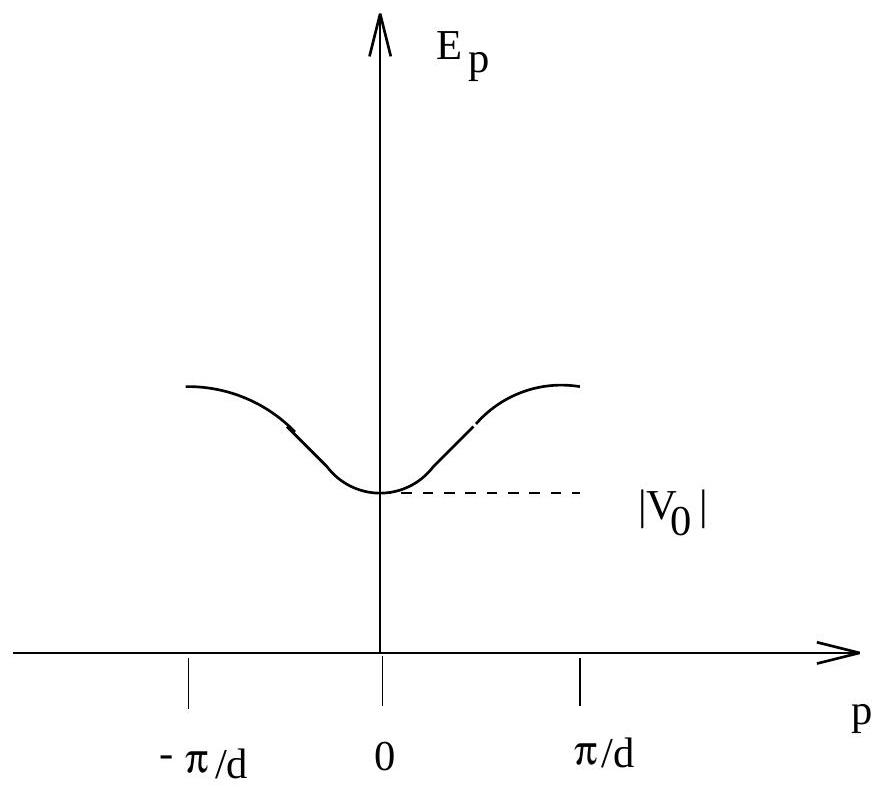
\includegraphics[max width=\textwidth]{2024_01_29_bd91e6d395035e9decbag-3}
\end{center}

Figure 1: Energy versus momentum for the one-dimensional lattice problem.

Consider a proton (charge $e$ ) in a one dimensional harmonic oscillator potential with unperturbed Hamiltonian

$$
H_{0}=\frac{p^{2}}{2 m}+\frac{1}{2} m \omega^{2} x^{2}
$$

We add a small time-dependent electric field so that $H=H_{0}+V_{t}$ with

$$
V_{t}=\frac{e E x}{1+(t / \tau)^{2}}, \quad-\infty<t<\infty
$$

If the system is initially in the ground state at $t=-\infty$, what is the probability to observe it in the first excited state after a long time $(t=\infty)$ ?

Thus,

$$
{ }_{\infty}\langle 1 \mid 0\rangle_{-\infty}=\frac{e E}{i} \pi \tau e^{-\omega \tau} \frac{1}{\sqrt{2 m \omega}}=-\frac{i \pi \tau e E}{\sqrt{2 m \omega}} e^{-\omega \tau}
$$

Finally, the desired transition probability is

$$
P(1)=\left.\left.\right|_{\infty}\langle 1 \mid 0\rangle_{-\infty}\right|^{2}=-\frac{(\pi \tau e E)^{2}}{2 m \omega} e^{-2 \omega \tau}
$$
\subsection{}
We want to evaluate the desired transition probability using the formalism of time-dependent perturbation theory in the interaction picture. We have:
\begin{equation}
  \begin{aligned}
    P_{1} &= -\frac{i}{\hbar} \int_{-\infty}^{\infty} \mathrm{d} t\left\langle 1\left|V_{t}\right| 0\right\rangle e^{i \omega_{1, 0} t} \\
\end{aligned}
\end{equation}
\end{document}